
\chapter{Machine Learning}

The general idea behind machine learning is this: Given a set of data, a machine creates a model that can be used to predict relationships between the various datum. The reasons for using a machine is generally because the size of the dataset, as well as the necessary computational requirements needed to make these models, is well beyond what is reasonable for a human to do alone.

Most of machine learning can be broken up into three general subdisciplines:
\begin{itemize}
	\item Supervised Learning:
	\item Unsupervised Learning:
	\item Reinforcement Learning:
\end{itemize}

Machine learning breaks down each element of a dataset into a set of \textbf{features} which describe it and differentiate it from the other elements. The resultant model is a collection of \textbf{parameters} that describe the relationship between elements of the dataset. \textbf{Hyperparameters} are parameters used in running the algorithm which arrives at the aforementioned parameters, and are not considered parameters of the model themselves.

\subsection{Model-Based vs Instance-Based Learning}
Model-based learning involves finding optimal parameters and uses a training dataset for its construction. An example is Support Vector Machines (Section \ref{sub:svm}).

Instance-based learning involves using the whole dataset as the model. An example is $k$-Nearest Neighbors (Section \ref{sub:knn}).

\subsection{Shallow vs Deep Learning}
Shallow learning involves building a model that trains on the features and measures the changes in the model by how well it matched the corresponding label. Deep learning is used in neural network architectures, and involves models that can learn features of features. Each layer in a neural network is in some sense a "shallow learning" layer.

\section{Supervised Learning}
Supervised learning takes a set of labelled feature vectors and builds a model to predict unlabelled data. 



\subsection{Support Vector Machines}\label{sub:svm}
Support Vector Machines (SVM) classify data-points by drawing boundaries between them. These boundaries are called ``Hyperplanes" and slice the points in their feature vectors. The technical definition of a hyperplane is any flat affine subspace. The data points “support" the each of these planes. i.e those closest to each plane are optimized around. In the case of two classes $y_i \in {-1,1}$. The ideal plane is defined as
\begin{align}
		\B{wx}_i-b =0
\end{align}
Where $\B{w}$ is the weights vector, which is optimized for, $\B{x}_i$ is the feature vector, and $b$ is the offset. This plane separates the two classes based off of the sign of any feature vector put into this equation
\begin{align}
	y = \textrm{sign}(\B{wx}_i-b)
\end{align}
One should class should give positive values, and the other, negative values. Mathematically we look for each point to obey

\begin{align}
	\B{wx}_i-b &\ge +1 ~\textrm{if}~ y_i = +1.  \label{svm_planes_pos}\\
	\B{wx}_i-b &\le -1 ~\textrm{if}~ y_i = -1.  \label{svm_planes_neg}
\end{align}

The above equations define planes as shown in Figure \ref{fig:svm}. The closest points of either classes are a separated by a distance $2/ ||\B{w}||$. We want the plane to be maximally discriminating, which is equivalent to maximizing this distance, or equivalently, \emph{minimizing} $||\B{w}||$. Using quadratic programming optimization we typically look to minimize \cite{burkov}


\begin{align}\label{svm_loss}
||\B{w}||^2
\end{align}

SVMs that minimize this function are said to have \emph{hard-margin}s, since points that fall on the wrong side of the hyperplane are not considered in the minimization procedure. 

\begin{figure}
\centerline{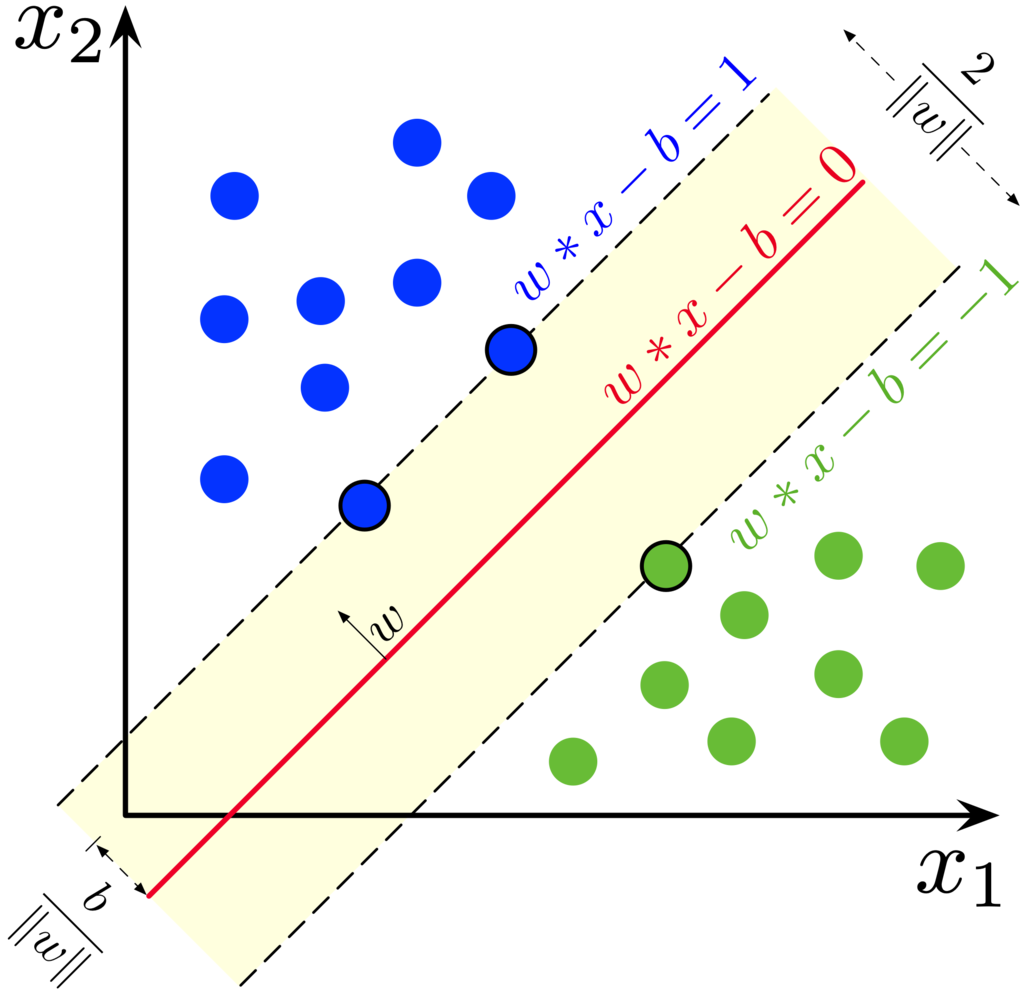
\includegraphics[width=0.5\linewidth]{mathematics/fig/svm.png}}
\caption{Maximum-margin hyperplane for an SVM trained with two classes \cite{wiki_svm}}
\label{fig:svm}
\end{figure}

\subsubsection{Hinge Loss}

If the classes are not cleanly distinguishable, which can happen if there is noise in the data, or the classes aren't entirely separable, one can look to minimize the \textbf{hinge loss function}, defined as
\begin{align}\label{hinge}
	C||\B{w}||^2 + \frac{1}{N}\sum_{i=1}^N \max(0,1-y_i(\B{wx}_i-b))
\end{align}
The first term in Equation \ref{hinge} is proportional to \ref{svm_loss}, while the second term is related to components on the wrong side of the boundary. Looking at Equations \ref{svm_planes_pos} and \ref{svm_planes_neg}, we see they are equivalent to 
\begin{align}
	y_i(\B{wx}_i-b) -1\ge 0\rightarrow 1- y_i(\B{wx}_i-b) \le 0
\end{align}
Therefore for any points on the correct side of the boundary, this expression is negative and $0$ is taken from the $\max$ function. However, if the point is on the \emph{wrong} side of the hyperplane, the loss function then has an added term proportional to how far away it is from the decision boundary.

SVMs that minimize the hinge loss are considered \emph{soft-margin}, since they allow for points fo fall on either side.

The choice of $C$ determines how much relative weight to give to the margin size (first term) and mislabelling (second term). A large $C$ gives a large margin which is good for generalizing the problem, while a small $C$  looks to classify the training data well.

\section{Decision Trees}
A decision tree is an acyclic graph that can be used to make decisions. Each ``leaf" of the tree assigns a label to the given feature vector. A balanced decision tree is one for which the questions split the groups into equal parts.

\subsection{Entropy}
Given $N$ different possible labels a feature vector could be associated to, we define $p_i$ with $i\in (1,N)$ as the proportion of any given label $i$. Using our full training dataset $D$, we can then define the entropy $S$ of the model as 

\begin{align}
	S^{(D)} = -\sum_{i=1}^N p^{(D)}_i\ln p^{(D)}_i
\end{align}

This tells us roughly how mixed up our dataset is. If the training data has two labels which are equally populated in the dataset, we have correspondingly larger energy than if we had only one of the labels show up. In the ideal case, each leaf of a decision tree will have just one label. A metric by which we can gauge how close we are to this ideal is by \emph{minimizing the entropy} of our model. 

There are a number of algorithms that that recursively split the dataset into those with smaller entropy i.e. $D\rightarrow D_1, D_2$. After doing this the effective entropy among the two independent datasets can be remeasured and compared with that before the split. This can then continue until a number of conditions are met such as you have only one kind of label, or there are no more splits that could further reduce the entropy.

\subsection{Boosted Decision Trees}
TODO
\subsection{Random Forests}
TODO
\subsection{Bootstrap Aggregation}
TODO


\section{Unsupervised Learning}
In unsupervised learning, the elements of the dataset are unlabelled, containing only feature vectors. This type of learning is useful for things like \textbf{clustering}, where the model looks to pair like-with-like, or \textbf{dimensionality reduction}, where the model translates a large set of features into a smaller set.


\subsection{Dimensionality Reduction}\label{dim_red}
When fitting to a high dimensional space, the model can become overfit and/or the correlation within the feature vectors can be overlooked. In order to reduce the feature vectors into a space which has more discriminating power, it is helpful to reduce the total dimensions of the problem at hand.
\subsubsection{Principal Component Analysis (PCA)}
Principal Component Analysis (PCA) turns our feature space into ``Principal Components", eigenvectors of our individual features. The analysis finds the dimension in the data that contains the most variance, thereby having the most discriminating power between events.

We first begin with our feature vectors
$$\mathbf{X} = \left.\left( 
                  \vphantom{\begin{array}{c}1\\1\\1\\1\\1\end{array}}
                  \smash{\underbrace{
                      \begin{array}{ccccc}
                             x_{00}&x_{10}&x_{20}&\cdots &x_{p0}\\
                             x_{01}&x_{11}&x_{21}&\cdots &x_{p1}\\
                             x_{02}&x_{12}&x_{22}&\cdots &x_{p2}\\
                             \vdots&&&\ddots&\\
                             x_{0n}&x_{1n}&x_{2n}&\cdots &x_{pn}
                      \end{array}
                      }_{p\text{ features}}}
              \right)\right\}
              \,n\text{ events}
$$\\

The idea is to shrink the dimensionality, so change $p\rightarrow l$ where $l$ is the desired dimensionality after PCA. 

We first start by normalizing each feature $k=1,\dots,p$ to have $\mu=0$ (centers the data) and $\sigma=1$ (accounts for different units).

\begin{align}
\mu_k = \frac{1}{n}\sum_{j=1}^n x_{kj} && \sigma_k^2 = \frac{1}{n-1}\sum_{j=1}^n (x_{kj}-\mu_k)^2 \\
\end{align}
It is worth noting the definition used by $\texttt{scikitlearn}$ only normalizes the mean, but not the standard deviation of each feature. We then redefine each column $k$ in the matrix with
\begin{align}
	\rho_{kj} = (x_{kj} - \mu_k)/\sigma_k
\end{align}
This gives us a new matrix
$$\mathbf{\tilde{X}} =  \left.\left( 
                  \vphantom{\begin{array}{c}1\\1\\1\\1\\1\end{array}}
                  \smash{\underbrace{
                      \begin{array}{ccccc}
                             \rho_{00}&\rho_{10}&\rho_{20}&\cdots &\rho_{p0}\\
                             \rho_{01}&\rho_{11}&\rho_{21}&\cdots &\rho_{p1}\\
                             \rho_{02}&\rho_{12}&\rho_{22}&\cdots &\rho_{p2}\\
                             \vdots&&&\ddots&\\
                             \rho_{0n}&\rho_{1n}&\rho_{2n}&\cdots &\rho_{pn}
                      \end{array}
                      }_{p\text{ features}}}
              \right)\right\}
              \,n\text{ events}
$$\\

Now we look at the Covariance matrix (Section \ref{covmat}) of each of our $p$ features, with
\begin{align}
\textbf{K}_{\rho_i,\rho_j} = \begin{pmatrix} 
                             \Cov[\rho_0,\rho_0]&\Cov[\rho_1,\rho_0]&\cdots &\Cov[\rho_p,\rho_0]\\
                             \Cov[\rho_0,\rho_1]&\Cov[\rho_1,\rho_1]&\cdots &\Cov[\rho_p,\rho_1]\\
                             \vdots&\vdots&\ddots&\vdots\\
                             \Cov[\rho_0,\rho_p]&\Cov[\rho_1,\rho_p]&\cdots &\Cov[\rho_p,\rho_p] \end{pmatrix}
\end{align}
This matrix will be symmetric, with $1$ along the diagonal (since we scale each feature to have a variance of 1). The next step is to diagonalize this matrix following Section \ref{diagonalize} and find it's eigenvalues $\lambda_i$ and eigenvectors $\textbf{a}_i = a_{ik}$. This puts the matrix into the form

$$\bf{K}' = \left(
{\begin{array}{cccc}
\lambda_0 & 0 &...&0 \\
0 & \lambda_1 & ...&0\\
\vdots & \vdots &\ddots & \vdots \\
0 & 0 & ... &\lambda_p
\end{array}}
\right)
$$

One can recognize now that in our new coordinate system, we have a new set of variables which each have a variance represented by the eigenvalue $\lambda_i$ itself. Because we want the most discriminating variable, we sort the eigenvectors and eigenvalues by the largest $\lambda_i$, which corresponds to the largest variance. Our new feature space is therefore
\begin{align}
	\rho_{ij} = a_{ik}\rho_{kj}
\end{align}
With $i=1,\dots,l$.


\section{Reinforced Learning}
Reinforced learning aims to try to maximize some numerical reward signal. The most important distinguishing feature is that it uses training information to evaluate actions taken rather than instruct which action to take \cite{sutton}.


\subsection{$k$-armed Bandits}
Slot machines are sometimes called "one-armed bandits" for the single lever they have together with their ability to steal money from peoples pockets. The idea behind $k$-armed bandits is to imagine instead of a single slot machine, you have $k$ of them. Each machine has a probability distribution of for hitting the "jackpot", and your job is to find out which one gives you the highest payoff.

Searching for the highest value machine involves a trade-off between $exploiting$ the information you have now and $exploring$ the space to look for something better you haven't found yet.

Greedy algorithms, in this case, use the lever which currently has the highest estimated chance of success. $\epsilon$-greedy algorithms do the same thing, but one in $\epsilon$ times, will select one of the levers at random instead to explore.


\subsubsection{Upper-Confidence-Bound Action Selection}

One can also use confidence bounds on the unknown probabilities to determine which lever to pull next. Because we don't want to miss out on a lever which could potentially be higher than the one we currently see is highest, we use the upper-confidence-bound when picking our current highest value estimate. To find the relevant confidence interval, we start with Hoeffding's Inequality (Section \ref{hoeffding}), which eventually tells us
\begin{align}
	A_t = \textrm{argmax}\Big[Q_t(a) + c\sqrt{\frac{\ln t}{N_t(a)}}\Big]
\end{align}
Where $A_t$ is the next action taken at time $t$ (i.e. iterations through the algorithm). $Q_t(a)$ is the expected value of action $a$ at time $t$. $c$ is the confidence level. $N_t(a)$ is the amount of times $a$ has been tried.

Overall, this tells us if an action $a$ is tried many times, $N_t(a)$ gets larger and the bound shrinks. Meanwhile, as time goes on, the bound itself grows to represent uncertainty in the system itself as to if it changes with time.


\subsection{Markov Decision Processes}
Markov Decision Processes (MDP) concerns using probability to optimize movement between "states". The framework proposes that the learning problem can be broken down into three signals that are passed back and forth: 
\begin{enumerate}
	\item Actions $A$
	\item States $S$
	\item Rewards $R$
\end{enumerate}
At present, how to represent states and actions is more of an art than a science \cite{sutton}. Rewards however are simple single numbers.



\section{Optimization}

\subsection{Metrics}
Different metrics are used to gauge the performance of a machine learning model

BLEU: bilingual evaluation understudy (used for evaluating language translation tasks).

\subsection{Cross-Validation}
TODO

\subsection{Gradient Descent}
Effectively a least-squares minimization technique (Section \ref{least-squares}) used to fit parametrized models to data. The algorithm uses an $n$-dimensional gradient which it recomputes given a set of parameters, which guides it towards a minimum of some kind (typically an error). 

In general, for large datasets, Gradient descent is slow.

TODO add linear fit gradient descent model.

\subsubsection{Minibatch Gradient Descent}
Cuts the data into "batches" for which the gradient can be computed much more easily than if one were to do the entire dataset.

\subsubsection{Stochastic Gradient Descent}
Among our entire dataset, a random selection of events are selected, for which gradient descent has its machinery run on. It is particularly good when there is redundancy in the data.

\subsection{Newton's Method}
Newton's method uses the second order Taylor expansion of the function to estimate the extremum in an optimization problem. This is contrasted with gradient descent which uses only the first order. Given a point $x_k$ where the optimizer is currently while looking for the extremum of $f(x)$, we have that
\begin{align}
	f(x_k+t)\approx f(x_k) + f'(x_k)t + \frac{1}{2}f''(x_k)t^2
\end{align}
If the second derivative $f''(x_k)$ is positive, the extremum of $f(x_k+t)$ will be when $f'(x_k+t) = d/dt f(x_k+t) = 0$ since $x=x_k+t$. This can be written as 
\begin{align}
	\frac{d}{dt}\Big( f(x_k) + f'(x_k)t + \frac{1}{2}f''(x_k)t^2\Big) = f'(x_k)+f''(x_k)t = 0 
\end{align}
Therefore under these conditions, $t = -f'(x_k)/f''(x_k)$ and the we assign the best estimate for the extremum of the function as
\begin{align}
	f(x_{k+1}) = f(x_k)-\frac{f'(x_k)}{f''(x_k)}
\end{align} 


\subsection{$k$-Nearest Neighbors}\label{sub:knn}
One of the simpler machine learning algorithms, $k$-nearest neighbors (KNN) takes in a new event (with it's own set of features) and finds the  $k$ events in the training data which it is closest to. This distance definition is adjustable. Once all the neighbors have been found, each votes on how to classify the new event.

This distance metric generally scales exponentially when new dimension are introduced, so it is advised to run dimensionality reduction (Section \ref{dim_red}) if using KNN for a high dimensional dataset.
\subsection{Naive Bayes}
When trying to deduce the probability of something dependent on many features $X_i$ conditional on something $S$, the naive way to do it is to assume they are all independent of each other
\begin{align}\label{naive_bayes}
	P(X_1,X_2,\dots,X_n|S) = P(X_1|S)P(X_2|S)\dots P(X_n|S)
\end{align}
This is the assumption made in Naive Bayes, for which computing the right side of Equation \ref{naive_bayes} is much easier than when one would need to look out for correlations.

When estimating $P(X_i|S)$ it is typical to use a \textit{pseudocount} for it's estimate so we don't assign 0 or 1 to the probability and bias our results. According to \cite{sutton} this is
\begin{align}
	P(X_i|S) = (k+\textrm{number~of~} S's\textrm{~with~} X_i's) / (2k+\textrm{number~of~} S \textrm{~total})
\end{align}


\subsection{Learning Rate}
TODO

\subsection{Step Size}
When iterating through a machine learning algorithm, the "step-size" determines how quickly you change your state from where you start from. The way of doing this is somewhat of an art, with a multitude of options such as 
\begin{itemize}
	\item Constant step size
	\item Step size which decreases as you make more iterations
\end{itemize}
\todo{ Add examples in \cite{sutton} with Reinforcement learning step sizes.}

\subsection{Loss Functions}
TODO
\subsubsection{Sum of Squared Residuals}
TODO

\subsection{Ant Colony Optimization}
TODO

\section{Neural Networks}
Neural networks are composed of perceptrons which approximates a single neuron. The network itself is composed of layers of these perceptrons which each take a set number of inputs, do a calculation based off of the inputs they are given, then ship out the output which is then used by other perceptrons.

Technically they are parametric nonlinear function approximators that can be fit to data to learn functions from input vectors to output vectors.

\subsection{Feed Forward Networks}
A feed forward network only has neurons which take inputs from the previous layer and pass them to the next layer. Consider $m$ total layers and the following definitions \cite{brilliant_backpropagation}
\\
\begin{tabular}{ l c }
  $r_k$ & number of neurons on layer $k\in[1,m]$\\
  $w_{ij}^k$ & weight given to output of neuron $j$ used in neuron $i$ on layer $k$  \\
  $b_i^k$ & bias used in neuron $j$ on layer $k$   \\
  $a_i^k$ & the product sum plus bias (activation) for node $i$ on layer $k$  \\
  $o_i^k$ & the output of neuron $i$ on layer $k$ \\
  $g$ & activation function for the hidden layer neurons \\
  $g_o$ & activation function for the output layer neurons \\
\end{tabular}\\
\\
Explicitly, the activation is written as
\begin{align}
	a_i^k =b_i^k + w_{ij}^ko_j^{k-1}
\end{align}
With summation implied following Einstein notation (Section \ref{einstein_notation}) and $j\in [1,r_{k-1}]$. If we defined 
\begin{align}
	w^k_{0i}=b_i^k && o_0^{k-1}=1
\end{align}
We can simplify the sum with
\begin{align}\label{nn_activation}
	a_i^k = w_{ij}^ko_j^{k-1}
\end{align}
with $j\in [0,r_{k-1}]$.

\subsection{Backpropagation}
To calculate the correct weights to assign to each neuron in the network, we find how the error function $\mathcal{E}$ changes as we change each weight $w_{ij}^k$ and bias $b_i^k$. Using gradient descent, we look for

\begin{align}
	\frac{\partial \mathcal{E}}{\partial w_{ij}^k} 
\end{align}
Typically the error function $\mathcal{E}$ is the sum of squared errors, but not always. In this example that is what we will use
\begin{align}
	\mathcal{E} = \frac{1}{2}\sum_{d=1}^N (\hat{y}_d-y_d)^2 = \sum_{d=1}^N E_d
\end{align}
Where $N$ is the total amount of data points we are training on and $E_{d}$ is the error on a given data point. The subscript $d$ is omitted for conciseness for the remaining description. Here we also assume that the neural network only outputs one final number, although this could be changed if we add another summation to the error equation. We can evaluate the gradient using the chain rule with
\begin{align}\label{neural_net_error}
	\frac{\partial E}{\partial w_{ij}^k} = \frac{\partial E}{\partial a_{i}^k}\frac{\partial a_{i}^k}{\partial w_{ij}^k}
\end{align}
The second term is easily computed using Equation \ref{nn_activation} with
\begin{align}
	\frac{\partial a_{i}^k}{\partial w_{ij}^k} = o_j^{k-1}
\end{align}
The first term is usually called the \textbf{error}, defined as 
\begin{align}
	\delta_{i}^k \equiv \frac{\partial E}{\partial a_{i}^k}
\end{align}
Looking first at the output layer $m$ and it's activation function $g_o$, we see
\begin{align}
	\delta_{i}^m \equiv \frac{\partial E}{\partial a_{i}^m} &= \frac{\partial}{\partial{a_{i}^m}}~\frac{1}{2} \Big(g_o(a_{i}^m)-y\Big)^2\\
	&= \Big(g_o(a_{i}^m)-y\Big)g_o'(a_{i}^m)
\end{align}
Therefore for the output layer we have
\begin{align}
	\frac{\partial E}{\partial w_{ij}^m} = \delta_{i}^m o_j^{m-1}
\end{align}


The reason why this method is called \textbf{backpropagation} is because the $\delta_i^m$ term from the last layer is then propagated backwards through the network to adjust weights in the other neurons. Let us next look for the change in layer $m-1$
\begin{align}
	\delta_j^{m-1} \equiv \frac{\partial E}{\partial a_{j}^{m-1}} &= \frac{\partial}{\partial{a_i^{m-1}}}\frac{1}{2}\Big(g_o(a_{i}^m)-y\Big)^2 \\
	&=\Big(g_o(a_{i}^m)-y\Big)g_o'(a_{i}^m)\frac{\partial a_{i}^m}{\partial a_{j}^{m-1}}\\
	&= \delta_i^m \frac{\partial a_{i}^m}{\partial a_{j}^{m-1}}
\end{align}
We can then recognize that
\begin{align}
	o_j^{k-1} &= g(a_j^{k-1})
\end{align}
which implies
\begin{align}
	a_i^m = w_{ij}^m g(a_j^{m-1})
\end{align}
Therefore we have
\begin{align}
	\frac{\partial a_{i}^m}{\partial a_{j}^{m-1}} = w_{ij}^m g'(a_j^{m-1})
\end{align}
And thus we have a recursive relation with
\begin{align}
	\delta_j^{k-1} = \delta_i^k w_{ij}^k g'(a_j^{k-1})
\end{align}
Which gives us the gradient for an arbitrary hidden layer with
\begin{align}
	\frac{\partial E}{\partial w_{ij}^k} = \delta_j^{k}o_i^{k-1} = \delta_l^{k+1} w_{lj}^{k+1} g'(a_j^{k})o_j^{k-1}
\end{align}
The weights are then adjusted using gradient descent with
\begin{align}
	\Delta w_{ij}^k = -\alpha~  \frac{\partial E}{\partial w_{ij}^k}
\end{align}

\subsection{Convolutional Neural Networks}
TODO

\subsection{Recurrent Neural Networks}
TODO

\subsection{Long-Short Term Memory (LSTM) Networks}
TODO

\subsection{Encoders and Decoders}
Take two different sequences of data, for instance an English sentence composed of words $x_i$ with $i\in (1,N)$ and it's corresponding translation into French words $y_j$ with $j\in(1,M)$.

The encoder transforms the input sequence of words $x_i$ into something called a context vector (e.g. One-Hot encoding). Context vector is then feed to the decoder, which uses the context vector together with the previously generated symbol of the output sequence. 

\subsection{Attention}

The general idea here is the colloquial usage of attention, where you have to choose what things to pay attention to. Deep nets generally react more strongly to parts of the data than others which is effectively the network selecting what it should pay attention to (e.g. the network may look at spots to look for a leopard over a jaguar).



From Wikipedia: ``In the context of neural networks, attention is a technique that mimics cognitive attention. The effect enhances the important parts of the input data and fades out the rest -- the thought being that the network should devote more computing power on that small but important part of the data. Which part of the data is more important than others depends on the context and is learned through training data by gradient descent. "


\subsection{Transformers}
TODO

\url{https://jalammar.github.io/illustrated-transformer/}

